\documentclass{article}

\usepackage{graphicx}
\usepackage{tikz}
\usepackage{tikzsymbols}
\usetikzlibrary{calc,patterns,shapes.geometric}
\pagestyle{empty}
\usepackage[margin=0pt]{geometry}
\geometry{papersize={14in,12in}}

\def\centerarc[#1](#2)(#3:#4:#5){\draw[#1] ($(#2)+({#5*cos(#3)},{#5*sin(#3)})$) arc (#3:#4:#5);}

\begin{document}
	\begin{figure}
		\centering
		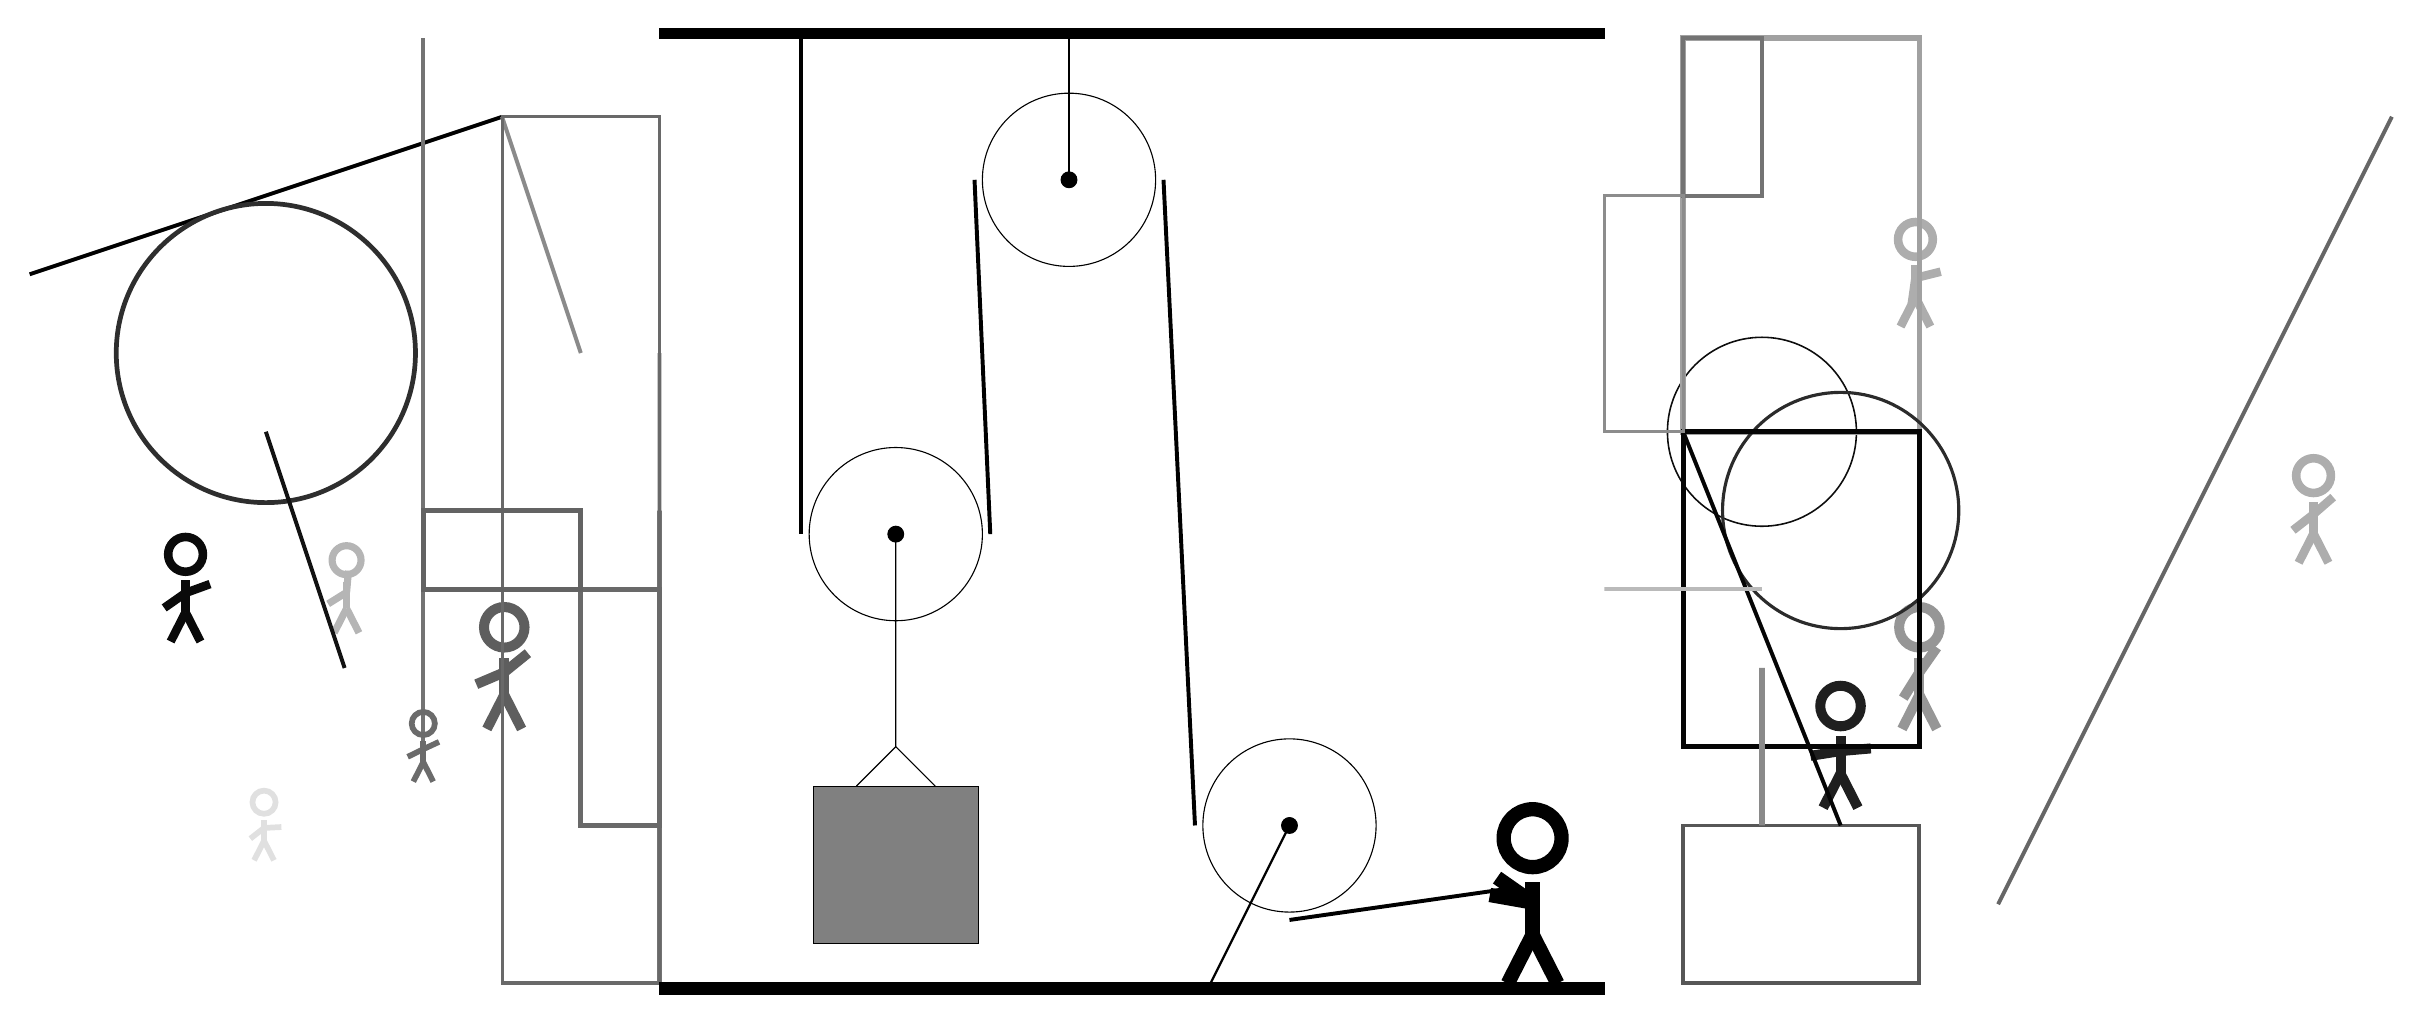
\begin{tikzpicture}
			%%%%% START %%%%%
			
			\draw[fill=black] (-2, 9) rectangle (10, 9.125);
			
			\draw[line width=0.5mm, color=black!100](-4, 8) -- (-10, 6);
			
			\node[line width=0.3mm, color=black!63] at (-4, 1) {\Strichmaxerl[7][23][39]};
			\node[line width=0.7mm, color=black!32] at (14, 6) {\Strichmaxerl[6][82][14]};
			\draw[line width=0.5mm, color=black!55](-5, 0) -- (-5, 9);
			\draw [line width=0.6mm, color=black!82](-7, 5) circle (1.9);
			\draw[line width=0.5mm, color=black!60](15, -2) -- (20, 8);
			\node[line width=0.5mm, color=black!12] at (-7, -1) {\Strichmaxerl[4][38][3]};
			\draw[line width=0.5mm, color=black!66] (11, -3) rectangle (14, -1);
			\node[line width=0.3mm, color=black!41] at (14, 1) {\Strichmaxerl[7][58][55]};
			
			\node[line width=0.7mm, color=black!88] at (13, 0) {\Strichmaxerl[7][9][5]};
			\draw[line width=0.6mm, color=black!21] (-2, 0) rectangle (-2, 5);
			\draw [line width=0.2mm, color=black!95](12, 4) circle (1.2);
			\draw[line width=0.7mm, color=black!37] (11, 9) rectangle (14, 4);
			
			\draw [line width=0.4mm, color=black!83](13, 3) circle (1.5);
			\node[line width=0.7mm, color=black!58] at (-5, 0) {\Strichmaxerl[4][26][25]};
			\draw [line width=0.6mm, color=black!24](-5, 6) circle (0.0);
			
			\node[line width=0.3mm, color=black!29] at (-6, 2) {\Strichmaxerl[5][32][85]};
			
			\draw[line width=0.6mm, color=black!55] (-2, -3) rectangle (-2, 3);
			\draw[line width=0.5mm, color=black!46](-4, 8) -- (-3, 5);
			\node[line width=0.4mm, color=black!96] at (-8, 2) {\Strichmaxerl[6][35][20]};
			\draw[line width=0.4mm, color=black!59] (-4, -3) rectangle (-2, 8);
			\draw[line width=0.6mm, color=black!98] (11, 0) rectangle (14, 4);
			\draw[line width=0.6mm, color=black!59] (-3, -1) rectangle (-2, 2);
			\node[line width=0.3mm, color=black!32] at (19, 3) {\Strichmaxerl[6][38][41]};
			\draw[line width=0.5mm, color=black!55] (12, 7) rectangle (11, 9);
			
			\draw[line width=0.5mm, color=black!93](-7, 4) -- (-6, 1);
			\draw[line width=0.5mm, color=black!98](11, 4) -- (13, -1);
			\draw[line width=0.4mm, color=black!45] (10, 7) rectangle (11, 4);
			
			\draw[line width=0.5mm, color=black!27] (12, 2) rectangle (10, 2);
			\draw[line width=0.6mm, color=black!61] (-3, 2) rectangle (-5, 3);
			\draw[line width=0.7mm, color=black!46] (12, -1) rectangle (12, 1);
			
			
			\draw (3.2, 7.2) circle (1.1);
			\draw[fill=black] (3.2, 7.2) circle (0.1);
			\draw[thick] (3.2, 7.2) -- (3.2, 9);
			
			\draw (6, -1) circle (1.1);
			\draw[fill=black] (6, -1) circle (0.1);
			\draw[thick] (6, -1) -- (5, -3);
			
			\draw (1, 2.7) circle (1.1);
			\draw[fill=black] (1, 2.7) circle (0.1);
			
			\draw (1, 2.7) -- (1, 0) -- (0.5, -0.5);
			\draw (1, 0) -- (1.5, -0.5);
			\draw[fill=black!50] (-0.05, -0.5) rectangle (2.05, -2.5);
			
			\draw[line width=0.5mm] (-0.2, 9) -- (-0.2, 2.7);
			\centerarc[line width=0.5mm](1, 2.7)(180:360:1.2000000000000002);
			\draw[line width=0.5mm](2.2, 2.7) -- (2.0, 7.2);
			\centerarc[line width=0.5mm](3.2, 7.2)(0:180:1.2000000000000002);
			\draw[line width=0.5mm](4.4, 7.2) -- (4.8, -1);
			\centerarc[line width=0.5mm](6, -1)(180:270:1.2000000000000002);
			\draw[line width=0.5mm](6, -2.2) -- (8.8, -1.8);
			
			\node at (9, -1.9) {\Strichmaxerl[10][-35][170]};
			
			\draw[fill=black] (-2, -3) rectangle (10, -3.15);
			
			%%%%% END %%%%%
		\end{tikzpicture}
	\end{figure}	
\end{document}